\documentclass[a4paper]{article}
\usepackage{exercise}
%um nur aufgaben zu zeigen
%\usepackage[noanswer]{exercise} 
\usepackage{../images/preamble}
\usepackage{rotating}
\usetikzlibrary{decorations.pathmorphing}
\usetikzlibrary{decorations.markings}
\usetikzlibrary{arrows}
\usetikzlibrary{shapes.geometric}
\newcommand{\midarrow}{\tikz \draw[-triangle 90] (0,0) -- +(.02,0);}
\usepackage{xcolor}
%\usepackage{draftwatermark}
%\SetWatermarkText{\textsc{Draft 2}}
%\SetWatermarkScale{3}
%\SetWatermarkColor{red!30}


\usepackage[printwatermark]{xwatermark}
%\newsavebox\mybox
%\savebox\mybox{\tikz[color=red,opacity=0.3]\node{\textsc{Entwurf}};}
%\newwatermark*[
%allpages,
%angle=45,
%scale=10,
%xpos=-4cm,
%ypos=4cm
%]{\usebox\mybox}
\pagestyle{fancy}
\fancyhead[L]{
\includegraphics[width=2cm]{../images/logo_scaled.pdf}}
\fancyhead[R]{\textsc{Aufgabenserie 7}}


\begin{document}
	\vspace*{-1cm}
	\parbox{4cm}{\vspace{-0.2cm}
\includegraphics[width=5cm]{../images/logo_scaled.pdf}}
	\parbox{10.6cm}{\setstretch{2.0} \centering{ \huge \textsf{Aufgabenserie 7
			}}\\
			%Abgabe: 8. April 2018 \\ 
			\vspace*{0.3cm} }
		\vspace{0.5cm}

\thispagestyle{empty}
\begin{framed}
	\noindent
	\scriptsize
	 Lösungen könnt ihr an \href{mailto:physikrolf@gmail.com}{physikrolf@gmail.com} schicken.
	 Neue Aufgaben wird es dann vermutlich wieder Mitte Mai geben.
	 \\ Die aktuellen Aufgaben sowie alle alten Aufgabenserien findet ihr auch auf \url{pankratius.github.io/rolf}.
\end{framed}

\noindent

\begin{Exercise}[title = Seilkraft, origin = {Morin - Classical Mechanics}, difficulty = 3, label = pucks]
Gegeben sei ein Pendel der Länge $\ell$ mit maximalem Auslenkungswinkel $A$, wobei $A \ll 1$. Für den Auslenkungswinkel $\theta(t)$ und die Winkelgeschwindigkeit $\omega(t)$ gilt
\begin{subequations}\label{averagetension:simpleharmonic}
	\begin{equation}\label{averagetension:angle}
		\theta(t) = A\cos\left(\omega_0t\right)
	\end{equation}
	\begin{equation}\label{averagtension:angularvel}
		\omega(t) = -A\omega_0\sin\left(\omega_0t\right),
	\end{equation}
\end{subequations}
wobei $\omega_0 = \sqrt{g/\ell}$ die Kreisfrequenz der Schwingung ist.\\
Bestimme näherungsweise (besser als $mg$!) die durchschnittliche Spannung im Faden während eines Umlaufs.
\end{Exercise}

\begin{Answer}
%	\begin{figure}[h]
%		\centering 
%		\begin{tikzpicture}
%		\draw[very thick](-.5,0) -- (.5,0);
%		\draw(0,0) -- (295:1.5);
%		\draw[dashed](0,0) -- (0,-1.5);
%		\node at (282:.6) {$\theta$};
%		\filldraw[black] (295:1.5) circle (1pt);
%		\draw[->] (295:1.5) -- (295:2);
%		\draw[->] (295:1.5) -- 
%		\end{tikzpicture}
%	\end{figure}
	Sei $F_s$ die Spannkraft im Seil. Dann ergibt Gleichung für das radiale Kräftegleichgewicht
	\begin{align}\label{averagetension:averagetension}
		F_s(t) &= m\omega(t)^2\ell + mg\cos \theta(t)\nonumber \\
		\implies 
		F_s(t) &= m \left(-A\omega_0 \sin(\omega_0 t)\right)^2 \ell + mg \cos \left(A \cos (\omega_0 t)\right).
	\end{align}
	Da wir nur kleine Auslenkungen betrachten, können wir die Taylor-Näherung des Cosinus für kleine Winkel betrachten, $\cos \alpha \approx 1 - \alpha^2/2$. Damit können wir $\cos\left(A \cos (\omega_0t)\right)$ nähern zu
	\[
	\cos\left(A\cdot \cos(\omega_0t)\right) \approx 1 -\frac{1}{2} A^2 \cos^2(\omega_0 t).
	\]
	Damit können \eqref{averagetension:averagetension} umformen zu
	\[
	F_s(t) \approx mA^2\omega_0^2\sin^2(\omega_0t) + mg\left(1- \frac{1}{2}A^2 \cos^2(\omega_0t)\right)
	\]
	Gleichzeitig können wir jetzt den Ausdruck für $\omega_0$ aus der Aufgabenstellung einsetzen, und erhalten schlussendlich
	\[
	\boxed{F_s(t) \approx mg + mgA^2 \left( \sin^2(\omega_0 t) - \frac{1}{2}\cos^2(\omega_0 t)\right).}
	\]
	Wir sehen nun, dass wir $F_s(t)$ besser als $mg$ abschätzen können, es gibt ja noch den zweiten Term in der Summe. Den Durchschnitt können wir jetzt über ein Integral ausrrechnen, wobei wir die Substitution $x:= \omega_0t$ nehmen können
	\begin{align*}
	\overline{F_s} &= mg + mgA^2\cdot\frac{1}{2\pi} \int_{0}^{2\pi} \sin^2(x) - \frac{1}{2}\cos^2(x)~dx\\
	&\boxed{= mg + \frac{mgA^2}{4}.}
	\end{align*}
\end{Answer}

\begin{minipage}[b]{0.5\textwidth}
\begin{Exercise}[label = resistancesquare, origin = EstPho 2012, title  =Widestandsquadrat, difficulty = 3]
In dem abgebildeten Stromkreis seien die Diagonalverbindungen nicht miteinander verbunden und es gelte $R_1 = R_2 = R_3 = R_4 =: R$ und $U_1 = U_2 =: U$.\\
Wie groß sind die Ströme $I_1, I_2, I_3, I_4$ durch die jeweiligen Widerstände?
\end{Exercise}
\end{minipage}
\hfill
\begin{minipage}[b]{0.5\textwidth}
	\centering
	\begin{tikzpicture}
		\draw (0,0) to [/tikz/circuitikz/bipoles/length=20pt, R] (2,0) to [/tikz/circuitikz/bipoles/length=20pt, R](2,2) to [/tikz/circuitikz/bipoles/length=20pt, R] (0,2) to [/tikz/circuitikz/bipoles/length=20pt, R] (0,0);
		\draw (0,0) to [/tikz/circuitikz/bipoles/length=20pt, battery1] (1,1) to (2,2);
		\draw (2,0) to[/tikz/circuitikz/bipoles/length=20pt, battery1] (1,1) to (0,2);
		\node at (-.3,1) {$R_1$};
		\node at (2.3,1) {$R_3$};
		\node at (1,2.3) {$R_2$};
		\node at (1,-.3) {$R_4$};
		\node at (.4,.8) {$U_1$};
		\node at (1.6,.8) {$U_2$};
	\end{tikzpicture}

\end{minipage}

\begin{minipage}[b]{0.6\textwidth}
\begin{Exercise}[title = Wärmezufuhr, origin = 1. IPhO 1967, difficulty = 4, label = balls]
Die homogenen Kugeln $A$ und $B$ seien komplet identisch und haben die gleiche Anfangstemperatur. Die Kugel $A$ hängt an einem Faden von einer Decke, und die Kugel $B$ liegt auf einer horizontalen Ebene.\\
Nun wird beiden Kugeln die gleiche Menge Energie in Form von Wärme hinzugefügt, wobei sämtliche Verluste an die Umgebung vernachlässigbar seien. Wie verhalten sich die Endtemperaturen der beiden Kugeln danach?
\end{Exercise}
\end{minipage}
\begin{minipage}[t]{0.4\textwidth}
	\centering
	\begin{tikzpicture}
	\draw[very thick] (-4,0) -- (-2,0);
	\draw (-3,0) -- (-3,-.5);
	\draw (-3,-1) circle (.5);
	\node at (-3,-1)  {$A$};
	\draw[very thick] (0,-2.2) -- (2,-2.2);
	\draw (1,-1.7) circle (.5);
	\node at (1,-1.7) {$B$}; 
	\end{tikzpicture}
\end{minipage}

\begin{Answer}
	\begin{figure}[h]
		\centering
		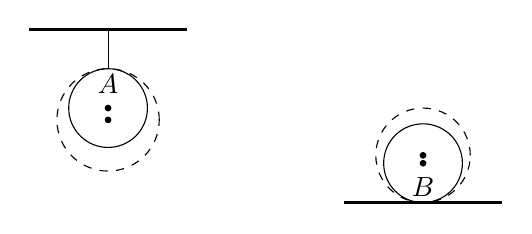
\begin{tikzpicture}
		\draw[very thick] (-4,0) -- (-2,0);
		\draw (-3,0) -- (-3,-.5);
		\draw (-3,-1) circle (.5);
		\draw[dashed](-3,-1.15) circle (.65);
		\node at (-3,-.7)  {$A$};
		\filldraw[black] (-3,-1) circle (1pt);
		\filldraw[black] (-3,-1.15) circle (1pt);
		\draw[very thick] (0,-2.2) -- (2,-2.2);
		\draw (1,-1.7) circle (.5);
		\draw[dashed] (1,-1.6) circle (.6);
		\filldraw[black] (1,-1.7) circle (1pt);
		\filldraw[black] (1,-1.6) circle (1pt);
		\node at (1,-2) {$B$}; 
		\end{tikzpicture}
	\end{figure}\\
	Durch die Wärmezufuhr dehnen sich die Kugeln aus. Gehen wir davon aus, dass die Kugel die Wärme langsam und aus allen Richtungen gleichmäßig verteilt zugeführt bekommt, können wir davon ausgehen, dass sich die Kugel auch gleichmäßig ausdehnt. Das bedeutet aber, dass sie ihre Form weiterhin beibehält.\footnote[2]{Vermutlich ist dies eine Folge der Rotationssymetrie der Anordnung und der gleichmäßigen Wärmezufuhr.}
	Dadurch verschiebt sich nun aber der Kugelschwerpunkt. Es kann sich jedoch der Schwerpunkt der Kugel $A$ nur nach unten verschieben, und der Schwerpunkt der Kugel $B$ nur nach oben. \\
	Verschiebt sich der Kugelschwerpunkt ändert sich auch die potentielle Energie im Gravitationsfeld der Erde. \\
	Im Fall der Kugel $A$ verschiebt sich der Schwerpunkt nach unten. Das bedeutet aber, dass die potentielle Energie der Kugel geringer wird. \\
	Gleichzeitig verschiebt sich der Schwerpunkt der Kugel $B$ weiter nach oben. Dadurch erhöht sich aber die potentielle Energie der Kugel. \\
	Bei der Bewegung von Kugel $A$ kann diese \glqq verlorene\grqq{} potentielle Energie aber nicht einfach verschwinden, und bei der Kugel $B$ muss die \glqq gewonnen\grqq{} potentielle Energie irgendwo herkommen. \\
	An dieser Stelle kann man ein Energieerhaltungsargument machen, oder, wenn man genauer seien möchte, den \textit{1. Hauptsatz der Thermodynamik} verwenden. Wenn wir mit $Q$ die Wärme bezeichnen, die einer Kugel zugeführt wird, mit $U$ die in der Kugel gespeicherte Energie und mit $W$ die Arbeit, die die
\end{Answer}



\end{document}